\section{Buffered Write} \label{sec:conn:buf_write}

\subsection{Design}
As described in Section \ref{sec:proto-ds} there are many different ways to implement a buffer write protocol, or a
protocol that writes to a ring buffer. We decided that we want to allow for variable message sizes. That means 
in contrast to the send protocol presented in section \ref{sec:conn:send} we do not have a fixed maximum buffer size
that will always be consumed, but we will only use the space we actually need.

\paragraph{} As we discussed we have two distinct problems we need to solve to get a correct buffered write connection.

\begin{itemize}
  \item We need to signal to the receiver that we have written to the buffer and how much was written. This is tightly 
    coupled to \emph{how} we write the data. We implemented three different approaches for solving this, which we present
    in the \emph{Sending} section below.
  \item We need to signal to the sender whether there is enough space to write the message. We implemented both a \emph{push}
    and \emph{pull} based implementation in the \emph{Acknowledging} section below.
\end{itemize}


\subsubsection{Buffer} \label{sec:conn:write:buf}
\begin{figure}[!ht]
\begin{center}

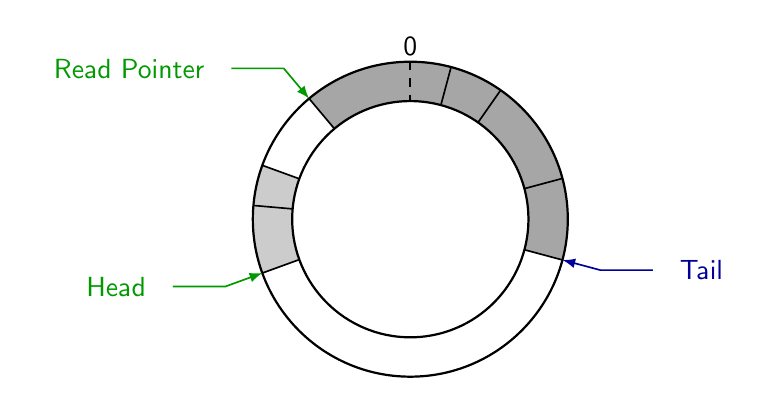
\begin{tikzpicture}[>=latex,font=\sffamily,semithick,scale=2]
    \fill [black!35] (0,0) -- (130:1) arc [end angle=-15, start angle=130, radius=1] -- cycle;

    \fill [black!20] (0,0) -- (200:1) arc [end angle=160, start angle=200, radius=1] -- cycle;
    \draw [thick] (0,0) circle (1cm);

    \node (zero) at (90:1.1) {0};
    \draw[dashed] (90:1) -- (0:0);
    \draw (200:1) -- (0:0);
    \draw (175:1) -- (0:0);
    \draw (160:1) -- (0:0);

    \draw (130:1) -- (0:0);
    \draw (75:1) -- (0:0);
    \draw (55:1) -- (0:0);
    \draw (15:1) -- (0:0);
    \draw (-15:1) -- (0:0);
    \node [circle,thick,fill=white,draw=black,align=center,minimum size=3cm] at (0,0) {};


    \draw [<-,black!40!green] (130:1) -- (130:1.25) -- +(-.333,0)
        node [black!40!green,left,inner xsep=.333cm] (rptr) {Read Pointer};
    \draw [<-,black!40!green] (200:1) -- (200:1.25) -- +(-.333,0)
        node [black!40!green,left,inner xsep=.333cm] (Head) {Head};
    \draw [<-,black!40!blue] (-15:1) -- (-15:1.25) -- +(.333,0)
        node [black!40!blue,right,inner xsep=.333cm] (Tail) {Tail};
\end{tikzpicture}

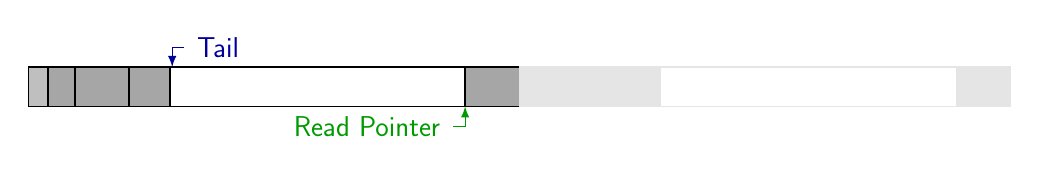
\begin{tikzpicture}[>=latex,font=\sffamily,every node/.style={minimum width=1cm,minimum height=1cm,outer sep=0pt,draw=black,semithick, scale=0.5}]
        \node [minimum width=.5cm, fill=black!25] at (0,0) (A) {};
        \node [anchor=west, minimum width=.68cm, fill=black!35] at (A.east) (B) {};
        \node [anchor=west, minimum width=1.38cm, fill=black!35] at (B.east) (C) {};
        \node [anchor=west, minimum width=1.03cm, fill=black!35] at (C.east) (D) {};
        \node [anchor=west, minimum width=7.5cm] at (D.east) (E) {};

        \node [anchor=west, minimum width=1.38cm, fill=black!35] at (E.east) (F) {};

        \node [anchor=west, minimum width=.5cm, fill=black!10, draw=none] at (F.east) (A') {};
        \node [anchor=west, minimum width=.68cm, fill=black!10, draw=none] at (A'.east) (B') {};
        \node [anchor=west, minimum width=1.38cm, fill=black!10, draw=none] at (B'.east) (C') {};
        \node [anchor=west, minimum width=1.03cm, fill=black!10, draw=none] at (C'.east) (D') {};
        \node [anchor=west, minimum width=7.5cm, draw=none] at (D'.east) (E') {};
        \node [anchor=west, minimum width=1.38cm, fill=black!10, draw=none] at (E'.east) (F') {};
        \node [anchor=west, minimum width=12.47cm, draw=black!10] at (F.east) (A') {};

        \draw [<-,black!40!blue, scale=1] (1.7,.25) -- (1.7, .5)  -- +(.15,0)
        node [black!40!blue,right,inner xsep=.333cm, draw=none] (Tail) {\huge Tail};
        \draw [<-,black!40!green, scale=1] (5.42,-.25) -- +(0, -.25)  -- +(-.15,-.25)
        node [black!40!green,left,inner xsep=.333cm, draw=none] (Head) {\huge Read Pointer};

\end{tikzpicture}
\end{center}
\caption{Ring Buffer with twice mapped memory to allows DMA writes over the end}
\comment{Fix figure to include read pointer correctly}
\label{fig:ringbuffer}
\end{figure}

The core of our buffered read connection is a ring buffer. This buffer ensures that the sender always knows \emph{where} to 
write to. Figure \ref{fig:ringbuffer} shows the basis for our ring buffer that we use for all implementations.

\paragraph{} We use a buffer that allows us to write arbitrary message sizes. There are three relevant pointers. 
The \emph{tail} which points to the next free memory address, the \emph{head}, which points to  the end of the 
free memory region, and the \emph{read pointer} which points to the start of the next unprocessed message. 

\paragraph{} The tail is only stored and updated by the sender. The tail directly gives the sender the address to write the 
next message to. The only thing the sender needs to check is, if there is actually enough space in the buffer for the 
intended message. So it needs at least a semi regular update on the head position. We look into this problem in 
the \emph{Acknowledging} section below.

\paragraph{} Receiving is a little more involved. Similarly to how we implemented the receive buffer management in 
Section \ref{sec:conn:send} we want to have the notion of \emph{reading} which returns a pointer to the start of 
the next unread message and \emph{freeing} a message which allows us to reuse that section of the ring buffer. 

This is where the difference between the \emph{head} and the \emph{read pointer} becomes apparent. The read pointer points 
to the next message the receiver has not read, while the head points to the oldest message the receiver has not freed. Reading
and freeing messages should work while interleaving, so we need some kind of management of free buffer to update the head 
correctly.

We solve this in a very simple way by having a linked list containing the starting address of the received messages. When
reading we push the address to the end of the list. When freeing we remove it from the list. The head is always the first 
element in the list.

We should note that the length of the message has to be communicated in some way, which we will address in the section 
\emph{Sending} below.





\paragraph{"Magic" Buffer} One problem we encountered while using such a ring buffer for RDMA is that we cannot simply 
\emph{wrap around} the end of the buffer using DMA. So if we want to write a message that is larger then the space left until
the end of the buffer we either need to skip to the front of the buffer, wasting space, or perform two writes, which is 
significantly slower.

Figure \ref{fig:ringbuffer} shows the our problem. Message $A$ cannot be written in a single RDMA write as it consists of 
two distinct, not connected memory regions. We can solve this by using something that has been coined 
\emph{"Magic" ring buffer} \comment{By? rgiesen.wordpress.com? Someone else?}. The idea is to map the same physical twice,
so that the same physical memory is adjacent to itself in virtual memory. You can see a representation of this in the 
Figure above. We use \emph{shared memory segments} on Linux to achieve this memory layout.

With this change we can simply write over the end of the buffer and do not have to worry about wrapping around.

\subsubsection{Sending} \label{sec:conn:write:sender}
With the ring buffer described above, the sender always knows where to write the next message to. We still need to solve
the problem of notifying the receiver that we sent a message and communicate the size of this message.

\paragraph{}The sender and receiver interfaces stay exactly the same as presented in Section \ref{sec:conn:send}. We use the same 
monotonically increasing \code{wr\_id}s to wait for sends to complete. The freeing is explained in the buffer section
above. We implemented three different ways to send and receive


\paragraph{Write Immediate}

We introduced \emph{Write with Immediate} in Section \ref{sec:bg:write}, which basically allows us to implement our sending 
and receiving in a very similar way to the send connection presented in the last section.

\paragraph{} Write with Immediate sends a 32 bit value while also writing to the specified location. More importantly it 
consumes a receive buffer and creates a completion event at the receiver. This completion event also contains the number 
of bytes written. So by writing the message using write with immediate, we will generate a completion event at the receiver
which gives it the size of the message. The receiver can then immediately repost the received buffer and return the ring 
buffer segment. Through the in order guarantees of RDMA we know that the messages in the ring buffer will be in the same
order as the completion events in the queue. We can reuse both the receive buffer management and batching from the send 
connection.


\paragraph{Write Offset}

One key reason to use the write instead of send verb is that we do not need to generate a completion event at the receiver
and the common knowledge that writes are faster than sends~\cite{}\comment{Cite some papers that say this}. When we use 
write with immediate however, we expect the same performance as when using the send verb and we still need to handle receive
buffers and completion events. So we need other ways to notify the sender of incoming messages.

\paragraph{} One way to implement this is by having additional metadata that allows the receiver to notice incoming data.
We implement such a protocol with what we call \emph{Write Offset}. The idea is that together with each message, the sender
also updates a metadata region at the receiver containing the \emph{tail}. The receive can then notice new incoming messages
by polling this tail and comparing it to the \emph{Read Pointer}. We solve the problem of finding the size of the messages by
writing it in the first 4 bytes of the written segment.

\paragraph{} This means to send a message of size $s$ the sender prepends the size $s$ to the message and writes it to the
tail of the buffer. It then writes the updated tail to the metadata region at the sender. Of these two RDMA writes only the 
latter needs to be signaled and we can issue both of the work requests at the same time, mitigating the impact of having to 
perform two writes for a single message. The receiver will always poll its local copy of the tail. As soon as the tail does 
not equal it \emph{Read Pointer} it knows that there are outstanding messages. We can read the first 4 bytes to get the size
of the next message and can then read it and update the \emph{Read Pointer}.

\paragraph{} This connection has obvious drawbacks, as we need to issue two writes for a single message. But this way we 
circumvent the need of receive buffers and end up with a completely \emph{passive receiver}. We thought of other metadata
based implementations of buffered read. For example instead of pushing the tail update to the receiver with each write, the
receiver could actively pull the tail update using RDMA read when necessary. This could potentially outperform the push based
implementation in high bandwidth situations. We did however not implement and evaluate this pull based approach.


\paragraph{Write Reverse}

With our \emph{Write Reverse} connection implementation we are able to notify the receiver without an additional write or
consuming a receive buffer. We can do this by polling on the actual transmitted data. Previous work~\cite{herd, farm} has
shown that RDMA updates memory in increasing memory order, at least for any modern systems we know. This allows us to poll
on the highest memory address to check whether a transfer is complete.

\begin{figure}[!hb]
\begin{center}

\begin{tikzpicture}[>=latex,font=\sffamily,semithick,scale=2]
  \draw [draw=none, fill=black!20] (20:2) arc [end angle=95, start angle=20, radius=2] -- (95:1.75)  arc [end angle=20, start angle=95, radius=1.75] -- cycle;
  \draw [draw=none, fill=green!10] (95:2) arc [end angle=145, start angle=95, radius=2] -- (145:1.75)  arc [end angle=95, start angle=145, radius=1.75] -- cycle;
  \draw (160:2) arc [end angle=20, start angle=160, radius=2];
  \draw (160:1.75) arc [end angle=20, start angle=160, radius=1.75];

  \draw (145:2) -- (145:1.75);
  \draw (140:2) -- (140:1.75);
  \draw[decoration={
            text along path,
            text={0},
            text align={center},
            raise=0.15cm},decorate] (145:1.75) arc (145:140:1.75);
  \draw (100:2) -- (100:1.75);
  \draw[decoration={
            text along path,
            text={data},
            text align={center},
            raise=0.15cm},decorate] (140:1.75) arc (140:100:1.75);


  \draw (95:2)  -- (95:1.75);
  \draw[decoration={
            text along path,
            text={1},
            text align={center},
            raise=0.15cm},decorate] (100:1.75) arc (100:95:1.75);

  \draw [<-,black!40!blue] (95:2) -- (95:2.25) 
        node [black!40!blue,above,inner xsep=.333cm] (Tail) {Tail};

  \draw [<-,black!20!blue] (140:2) -- (140:2.25) 
        node [black!20!blue,above,inner xsep=.333cm] (ntail) {\small New Tail};



  \draw (60:2)  -- (60:1.75);
  \draw (55:2)  -- (55:1.75);

\end{tikzpicture}
\end{center}
\caption{Reversed Ring buffer}
\label{fig:write-rev}
\end{figure}

\paragraph{} So the core idea is to append a \emph{valid byte} at the end of the message on which the receiver can poll on.
There are two issues with introducing this two our existing ring buffer design.

\begin{itemize}
  \item The messages have variable size, so the receive does not know the location of this \emph{valid byte}.
  \item We need to zero this byte after freeing the buffer segment, potentially forcing us to zero the complete segment 
    which is fairly expensive.
\end{itemize}

We can solve both these problems by flipping our ring buffer. Instead of writing in increasing order, we add messages in 
decreasing order. Figure \ref{fig:write-rev} shows how writing a message works, the newly written message is highlighted in 
light green. We write a message structure of: 
A zero byte, followed by the data, the message length, and a valid byte, which is set to one. This has the effect that the
receiver can poll on the next byte in the ring buffer to check for new incoming messages and read the next 4 bytes to get 
the size of it. The prepended zero byte actually zeros the valid byte of the next massage. This means the receiver does not 
need to zero anything after freeing the segment.




We note that reversing the ring buffer does not really change any implementation details presented in 
Section~\ref{sec:conn:write:buf}. The double mapped memory trick still works and the freeing of buffers still works in a
similar way.

\subsubsection{Acknowledging}

We showed that there are multiple ways to transfer data and notify the sender. One other thing we need to prevent is for the
sender to overrun the ring buffer. That means the sender needs at leas a periodic update of the head position to decide if
there is space left to write to. We call this \emph{acknowledging} the head position.

We present two different approaches to do this. A pull based approach, where the sender reads the updated head from the
receiver, and a push based approach, where the receiver sends updates to the sender when the head position changes.

\paragraph{Pull} For the pull based implementation the receiver has a dedicated memory region where it writes the current 
head to. The sender has a cache of this head position. As soon as there is not enough space for the next message, given 
the cached head value, the sender will perform a RDMA read to update its cache.

Our current implementation will immediately block until the read succeeds. There is potential to optimize this by preemptively 
updating the head without waiting for it to complete. We experimented adding this, but as we did not see any significant 
performance improvements by adding this, we decided not to add this to reduce complexity. \comment{Maybe we should add it. Its ready}

\paragraph{Push} We also implemented a push based approach, where the receiver will send updates of the tail value using 
RDMA sends. To reduce the load of this acknowledgements we only send updates when the receiver has processed an eighth of 
the complete ring buffer. The sender will then poll its receive queue as soon as it cannot write the next message given its
cache of the tail value.

\subsection{Conclusion}

It is generally assumed that the Write verb is significantly faster than using Send and Receive. In this section we have 
shown that in the end when building a message passing interface using a ring buffer, the difference is not as pronounced.


\paragraph{} We have shown that buffered read connections achieve very similar, high performance than send receive connections
Using this protocol we can provide \emph{variable message size}, which allows transmission to only use the buffer space it 
actually needs. Depending on the approach we can have convenient \emph{interrupts} but compared to the send receive protocol
we need to give up some of the \emph{fairness} guarantees, as a single blocked message can halt the complete ring buffer.

\paragraph{} In our benchmarking we encountered some unintuitive results. Most notably the \emph{Write Reverse Anomaly} when 
sending message of size 4 KB or multiples of it. This again shows that RDMA based connections need to be designed carefully
and tested thoroughly to achieve the best performance.

\paragraph{} In the end Buffered Read connections give us good performance, work reliably, and utilizes the buffer space more
efficiently than using send receive verbs. They however give us very similar performance compared to the send receive 
connections and is significantly more involved to implement.









